Computerspiele nutzen Nebenläufigkeit und Multithreading seit dem Aufkommen von Mehrkern-Prozessoren, um eine bessere Performance zu erreichen~\cite{Davies2006}. Es gibt verschiedene für Spiele geeignete Multithreading-Architekturen, die jeweils eigene Vor- und Nachteile mit sich bringen. Im Folgenden werden zwei in der Computerspielindustrie weit verbreitete Multithreading-Architekturen betrachtet.

\subsubsection{\glsentrylong{sot}}
\begin{figure}
	\centering
	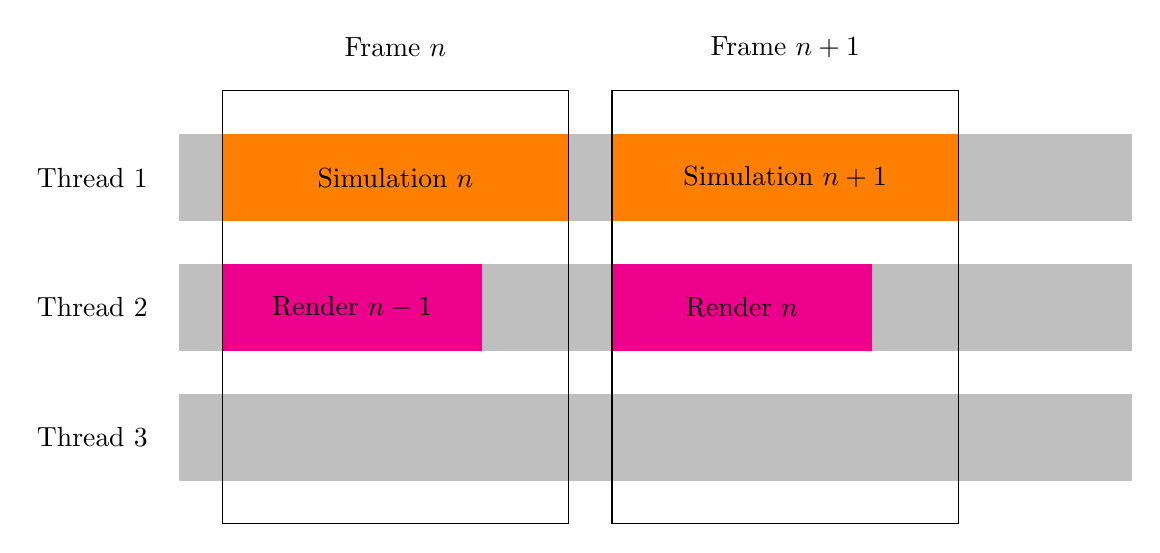
\begin{tikzpicture}[scale=1.1]
			\fill[lightgray]  (0,0) rectangle (11,1);
			\fill[lightgray] (0,-1.5) rectangle (11,-0.5);
			\fill[lightgray]  (0,1.5) rectangle (11,2.5);
			
			\node at (-1,2) {Thread 1};
			\node at (-1,0.5) {Thread 2};
			\node at (-1,-1) {Thread 3};
			
			
			\fill [orange] (0.5,2.5) rectangle (4.5,1.5);
			\fill [orange] (5,2.5) rectangle (9,1.5);
			\fill [magenta] (0.5,1) rectangle (3.5,0);
			\fill [magenta] (5,1) rectangle (8,0);
			
			
			\node at (2.5,2) {Simulation $n$};
			\node at (7,2) {Simulation $n+1$};
			\node at (2.5,3.5) {Frame $n$};
			\node at (7,3.5) {Frame $n+1$};
			
			\draw  (0.5,3) rectangle (4.5,-2);
			\draw  (5,3) rectangle (9,-2);
			
			\node at (2,0.5) {Render $n-1$};
			\node at (6.5,0.5) {Render $n$};

	\end{tikzpicture}
	\caption[Darstellung der Nutzung von Multithreading in \glsentrylong{sot}.]{Darstellung der Nutzung von Multithreading in \glsentrylong{sot}. Systeme laufen auf eigenen Threads. Es wird die Auslastung während zwei Frames $n$ und $n+1$ gezeigt. Einige Threads sind dadurch nicht zu \SI{100}{\percent} ausgelastet (graue Bereiche). In diesem Fall kann Thread 3 gar nicht genutzt werden. Thread 2 übernimmt das Rendering (magenta), durch Pipelining wird dabei immer der Zustand der Simulation (orange) des letzten Frames dargestellt. Abbildung nach \cite[S.~14]{Tatarchuk2014}}\label{fig:sot}
\end{figure}
Eine einfache Architektur vergibt, wie in Abbildung~\ref{fig:sot} gezeigt, für einzelne Systeme (wie Simulation oder Rendering) eigene Threads, die diese exklusiv nutzen~\cite{Davies2006,Tatarchuk2014,Genova2015,Hodgman2016}. \textcite{Tatarchuk2014} bezeichnet diese Architektur als \ac{sot}. Diese Architektur bietet einige Vor- und Nachteile, die nun erörtert werden.
\begin{itemize}
	\item[$+$] Die Architektur bietet den Vorteil, dass die Ausführung innerhalb der Systeme seriell ist, was die Entwicklung einfacher macht als nebenläufige Entwicklung, wie in Abschnitt~\ref{sec:nebenl-folgen} \nameref{sec:nebenl-folgen} beschrieben worden ist.
	\item[$+$] Solange die Systeme voneinander separiert sind, gibt es keine Probleme, die mit Nebenläufigkeit einhergehen, da beispielsweise Wettkampfbedingungen nur auftreten können, wenn nebenläufig auf geteilte Daten zugegriffen wird. Da keine Wettkampfbedingungen verhindert werden müssen, entfällt blockierende Synchronisierung und Deadlocks sind ausgeschlossen.
	\item[$-$] Auf heterogenen Plattformen, die beispielsweise unterschiedliche Prozessoreinheiten besitzen, kann es zu Performance Problemen kommen. Die Architektur muss eventuell für jede Plattform anders aufgebaut sein. Es existiert also eine gewisse Abhängigkeit von der Hardware.
	\item[$-$] Da immer Systeme existieren, die auf Daten anderer Systeme zugreifen, muss zur Synchronisierung der Systeme Pipelining (das im Folgenden erklärt wird) betrieben werden. Das erfordert einen großen Speicheraufwand, da alle Daten zwischengespeichert werden müssen. Dann können Systeme auf die Daten anderer Systeme zugreifen, ohne dass Wettkampfbedingungen befürchtet werden müssen.
\end{itemize}

\begin{figure}
	\centering
	\begin{tikzpicture}
		\begin{scope}[shift={(0,3.3)}]
			\node[minimum width = 2cm,minimum height = 6mm, fill=magenta!100!orange,anchor=west] at (0,0) (f1){Frame 1};
			\node[minimum width = 2cm,minimum height = 6mm, fill=magenta! 75!orange,anchor=west] at (f1.east) (f2){Frame 2};
			\node[minimum width = 2cm,minimum height = 6mm, fill=magenta! 50!orange,anchor=west] at (f2.east) (f3){Frame 3};
			\node[minimum width = 2cm,minimum height = 6mm, fill=magenta! 25!orange,anchor=west] at (f3.east) (f4){Frame 4};
			\node[minimum width = 2cm,minimum height = 6mm, fill=magenta!  0!orange,anchor=west] at (f4.east) (f5){Frame 5};
			\node[minimum width = 2cm,minimum height = 6mm, fill=magenta!100!orange,below = 3mm of f1] (r1){Frame 1};
			\node[minimum width = 2cm,minimum height = 6mm, fill=magenta! 75!orange,anchor=west] at (r1.east) (r2){Frame 2};
			\node[minimum width = 2cm,minimum height = 6mm, fill=magenta! 50!orange,anchor=west] at (r2.east) (r3){Frame 3};
			\node[minimum width = 2cm,minimum height = 6mm, fill=magenta! 25!orange,anchor=west] at (r3.east) (r4){Frame 4};
			\node[minimum width = 2cm,minimum height = 6mm, fill=magenta!  0!orange,anchor=west] at (r4.east) (r5){Frame 5};
			\node[anchor=east] at (f1.west) (s) {Simulation:};
			\node[anchor=east] at (r1.west) {Rendering:};

			\node[above = 1mm of s.north west, anchor=south west,] {Kein Pipelining:};

			\draw[->] (r1.south west) ++(0,-.2) -- ++(13,0) node[below] {Zeit};
		\end{scope}
		\node[minimum width = 2cm,minimum height = 6mm, fill=magenta!100!orange,anchor=west] at (0,0) (f1){Frame 1};
		\node[minimum width = 2cm,minimum height = 6mm, fill=magenta! 75!orange,anchor=west] at (f1.east) (f2){Frame 2};
		\node[minimum width = 2cm,minimum height = 6mm, fill=magenta! 50!orange,anchor=west] at (f2.east) (f3){Frame 3};
		\node[minimum width = 2cm,minimum height = 6mm, fill=magenta! 25!orange,anchor=west] at (f3.east) (f4){Frame 4};
		\node[minimum width = 2cm,minimum height = 6mm, fill=magenta!  0!orange,anchor=west] at (f4.east) (f5){Frame 5};
		\node[minimum width = 2cm,minimum height = 6mm, anchor=north, below = 3mm of f1] (r0){};
		\node[minimum width = 2cm,minimum height = 6mm, fill=magenta!100!orange,anchor=west] at (r0.east) (r1){Frame 1};
		\node[minimum width = 2cm,minimum height = 6mm, fill=magenta! 75!orange,anchor=west] at (r1.east) (r2){Frame 2};
		\node[minimum width = 2cm,minimum height = 6mm, fill=magenta! 50!orange,anchor=west] at (r2.east) (r3){Frame 3};
		\node[minimum width = 2cm,minimum height = 6mm, fill=magenta! 25!orange,anchor=west] at (r3.east) (r4){Frame 4};
		\node[minimum width = 2cm,minimum height = 6mm, fill=magenta!  0!orange,anchor=west] at (r4.east) (r5){Frame 5};

		\node[anchor=east] at (f1.west) (s) {Simulation:};
		\node[anchor=east] at (r0.west) {Rendering:};

		\node[ above = 1mm of s.north west,anchor=south west,] {Pipelining:};

		\draw[->] (r0.south west) ++(0,-.2) -- ++(13,0) node[below] {Zeit};
	\end{tikzpicture}
	\caption[Unterschied der Ausführung abhängig von der Nutzung von Pipelining.]{Unterschied der Ausführung abhängig von der Nutzung von Pipelining. Wird Pipelining genutzt, ist die Simulation dem Rendering immer einen Frame voraus.}\label{fig:pipelining}
 \end{figure}

Die Zwischenspeicherung wird insbesondere dann wichtig, wenn wie in Abbildung~\ref{fig:sot} sogenanntes \emph{Pipelining} betrieben werden soll. Das heißt, dass Systeme nicht gleichzeitig, sondern nacheinander ausgeführt werden. Nachdem ein Schritt fertig ist, beginnt allerdings gleich die Ausführung des nächsten Schritts. Damit ergibt sich bei zwei Systemen ein Bild wie in Abbildung~\ref{fig:pipelining}. Betrachtet man einen Zeitpunkt, also ein Bild (engl. Frame), so arbeiten alle Systeme gleichzeitig, aber an unterschiedlichen Daten. Während die Simulation die Daten für Frame $n$ berechnet, nutzt das Rendering-System die Daten von Thread $n-1$.

Für die Zwischenspeicherung kann ein sogenannter \emph{Double-Buffer}~\cite[S.~143]{Nystrom2015} genutzt werden. Das ist ein Puffer, der zwei Speicherstellen verwendet. So kann ein System Daten berechnen und in die eine Speicherstelle einfügen, während nebenläufig die andere Speicherstelle von anderen Systemen ausgelesen werden kann, ohne dass dort Daten verändert werden. Zu einem bestimmten Zeitpunkt werden dann die Speicherstellen getauscht, sodass immer eine Speicherstelle unverändert ist, während die andere Stelle beschrieben wird.

Die Nutzung von \ac{sot} bietet sich an, wenn nur für eine Plattform, beispielsweise eine Spielekonsole, entwickelt wird und es keine starken Speicherplatzrestriktionen gibt. Zudem ist die Implementierung einfacher als die der folgenden Architektur.

\subsubsection{Jobsystem}\label{sec:gamesJobsystem}

\begin{figure}
	\centering
	\begin{tikzpicture}[scale=1.1]
		\fill[lightgray]  (0,0) rectangle (11,1);
		\fill[lightgray] (0,-1.5) rectangle (11,-0.5);
		\fill[lightgray]  (0,1.5) rectangle (11,2.5);
		
		\node at (-1,2) {Thread 1};
		\node at (-1,0.5) {Thread 2};
		\node at (-1,-1) {Thread 3};
	
		\foreach \i in {0,3.5,7}{
		\fill [orange,draw=lightgray] ($(\i,0) + (0.5, 1.5)$) rectangle ($(\i,0) +(1.5, 2.5)$);
		\fill [orange,draw=lightgray] ($(\i,0) + (0.5,-1.5)$) rectangle ($(\i,0) +(1.5,-0.5)$);
		\fill [orange,draw=lightgray] ($(\i,0) + (1.5, 1.5)$) rectangle ($(\i,0) +(2.5, 2.5)$);
		\fill [orange,draw=lightgray] ($(\i,0) + (0.5, 0.0)$) rectangle ($(\i,0) +(1.5, 1.0)$);
		
		\fill [magenta,draw=lightgray] ($(\i,0) + (2.5, 1.5)$) rectangle ($(\i,0) + (3.5, 2.5)$);
		\fill [magenta,draw=lightgray] ($(\i,0) + (2.5, 0.0)$) rectangle ($(\i,0) + (3.5, 1.0)$);
		\fill [magenta,draw=lightgray] ($(\i,0) + (2.5,-1.5)$) rectangle ($(\i,0) + (3.5,-0.5)$);
		
		\draw  ($(\i,0) + (0.5,3)$) rectangle ($(\i,0) + (3.5,-2)$);
		
		\node[font=\footnotesize] at ($(\i,0) + (1,2)$) {Sim 1};
		\node[font=\footnotesize] at ($(\i,0) + (1,0.5)$) {Sim 2};
		\node[font=\footnotesize] at ($(\i,0) + (1,-1)$) {Sim 3};
		\node[font=\footnotesize] at ($(\i,0) + (2,2)$) {Sim 4};
		\node[font=\footnotesize] at ($(\i,0) + (3,2)$) {Ren 1};
		\node[font=\footnotesize] at ($(\i,0) + (3,0.5)$) {Ren 2};
		\node[font=\footnotesize] at ($(\i,0) + (3,-1)$) {Ren 3};
	
		}
	\node at (2,3.5) {Frame $n$};
	\node at (5.5,3.5) {Frame $n+1$};
	\node at (9,3.5) {Frame $n+2$};
	\end{tikzpicture}
	\caption[Darstellung der Nutzung von Multithreading mit einem Jobsystem.]{Darstellung der Nutzung von Multithreading mit einem Jobsystem. Die Systeme definieren Jobs, die frei auf die vorhandenen Threads aufgeteilt werden. Sim steht für Simulation und Ren für Rendering. Die Abbildung ist schematisch, die Jobs müssen nicht exakt die gleiche Länge haben, wobei jedoch kurze Jobs mit ähnlichen Laufzeiten ideal sind. Im Vergleich zu Abbildung~\ref{fig:sot} lässt sich eine höhere Auslastung der Threads erkennen, was wiederum höhere FPS zur Folge hat.}\label{fig:jobt}
\end{figure}
Eine etwas komplexere Architektur liefert die Implementierung eines sogenannten \emph{Job-} oder \emph{Task-Systems}~\cite{Davies2006,Tatarchuk2014,Genova2015,Hodgman2016}. Ein Schema der Architektur ist in Abbildung~\ref{fig:jobt} zu sehen. Anstatt Aufgaben fest auf einzelne Threads zu verteilen, gibt es \emph{Jobs} (beziehungsweise Tasks) und ein System, das die Jobs auf Threads verteilt. Konzeptuell entspricht die Architektur annähernd dem in Abschnitt~\ref{sec:executor} beschriebenen \class{ExecutorService} in Java. 

Die kurzen Jobs werden an das System übergeben. Das System verwaltet die Threads, deren Anzahl idealerweise der Anzahl der Hardware-Threads entspricht, da dann die Leistung des Prozessors optimal ausgenutzt werden kann und die Anzahl der Kontextwechsel minimiert wird. Ist ein Thread im Leerlauf, wird ein Job an den Thread zur Ausführung übergeben.

\begin{figure}
	\centering
	\begin{tikzpicture}
		\node[fill=orange] (sim1) {Sim 1};
		\node[fill=orange,below=of sim1] (sim2)  {Sim 2};
		\node[fill=orange,below=of sim2] (sim3)  {Sim 3};

		\node[fill=orange,right=of sim2] (sim4)  {Sim 4};

		\node[fill=magenta,right=of sim4] (ren2)  {Ren 2};
		\node[fill=magenta,above=of ren2] (ren1)  {Ren 1};
		\node[fill=magenta,below=of ren2] (ren3)  {Ren 3};

		
		\draw[->](sim1.east) -- (sim4.north west);
		\draw[->](sim2.east) -- (sim4.west);
		\draw[->](sim3.east) -- (sim4.south west);
		\draw[->](sim4.north east) -- (ren1.west);
		\draw[->](sim4.east) -- (ren2.west);
		\draw[->](sim4.south east) -- (ren3.west);
	\end{tikzpicture}
	\caption[Beispiel eines Job-Graphen in einem Jobsystem.]{Beispiel eines Job-Graphen, der der Ausführung in Abbildung~\ref{fig:jobt} zugrunde liegen könnte. Die farbigen Knoten stellen Jobs dar, wobei orange Knoten Simulations-Jobs und magentafarbene Knoten Rendering-Jobs sind. Die gerichteten Kanten zeigen die mögliche Ausführungsreihenfolge an. So muss beispielsweise Sim 4 nach Sim 3 ausgeführt werden. Gibt es keinen Pfad von Job $A$ zu Job $B$, so können beide parallel ausgeführt werden.}\label{fig:jobdependencies}
\end{figure}
Das System kann zudem so implementiert werden, dass es Abhängigkeiten zwischen einzelnen Jobs gibt, das heißt, dass ein Job beispielsweise erst ausgeführt wird, wenn ein anderer Job abgeschlossen ist. Daraus bildet sich ein Job-Graph, der die nebenläufige Ausführung der Jobs beschreibt. Es hat sich als hilfreich erwiesen, feste Synchronisationspunkte zu definieren, damit auf systemübergreifende Daten zugegriffen werden kann. Das kann im Jobsystem wie in Abbildung~\ref{fig:jobdependencies} durch Jobs repräsentiert werden, die Abhängigkeiten zu vielen vorangehenden Jobs sammeln und dann als Abhängigkeit für die folgenden Jobs dienen. Nun werden einige Vor- und Nachteile eines Jobsystems betrachtet.
\begin{itemize}
	\item[$+$]  Da die Durchführung von Jobs nicht an bestimmte Threads gekoppelt ist, kann Hardware mit mehr Prozessoreinheiten sofort voll ausgenutzt werden. Dadurch werden ohne zusätzlichen Programmieraufwand verschiedenste Plattformen unterstützt.
	\item[$+$] Ein Jobsystem bietet die Möglichkeit, Simulation und Rendering in einem Frame sequentiell durchzuführen, ohne alle Nebenläufigkeit zu verlieren. Durch das Jobsystem können die Systeme intern parallelisiert werden. Werden Simulation und Rendering sequentialisiert, ist es nicht nötig den Spielzustand zwischenzuspeichern, da die Simulation während des Renderings bereits abgeschlossen ist und somit Wettkampfbedingungen ausgeschlossen sind (da das Rendering nur lesend auf Daten zugreift). Damit benötigt man weniger Speicher als bei einer Architektur, die auf einen Zwischenspeicher angewiesen ist. Spiele, die ohnehin viel Speicher verbrauchen oder auf speicherbeschränkten Systemen ausgeführt werden sollen, können auf diese Art von Nebenläufigkeit Gebrauch machen. 
	
	Wie in Abbildung~\ref{fig:jobt} zu sehen, führt dies aber auch dazu, dass die Threads gegebenenfalls nicht vollständig ausgelastet sind, da beispielsweise alle noch auszuführenden Jobs auf die Beendigung eines noch nicht abgeschlossenen Jobs warten müssen.
	\item[$+$] Auch mit einem Jobsystem gibt es weiterhin die Möglichkeit mittels eines Zwischenspeichers Pipelining zu betreiben und so die in Abbildung~\ref{fig:jobt} sichtbaren Auslastungslücken zu schließen.
	\item[$+$] Wird ein neues System hinzugefügt, beispielsweise zur Verwaltung der Audioausgabe, muss die grundlegende Architektur nicht angepasst werden, um das neue System nebenläufig in das Spiel zu integrieren. Das System kann sofort Jobs erzeugen und diese zur Ausführung bringen.
	\item[$-$] Das Jobsystem basiert auf Jobs, die erstellt werden müssen. Soll also ein bestehendes Spiel ein Jobsystem nutzen, muss der gesamte Code so umgeschrieben werden, dass bestehende Abläufe in kleine Jobs aufgeteilt werden und dann mit den korrekten Abhängigkeiten nebenläufig ausgeführt werden. Es muss also tief in die bestehenden Systeme eingegriffen werden. Dieses Problem ergibt sich bei der \ac{sot} Architektur nicht, da hier die Systeme intern weiterhin sequentiell sind.
	\item[$-$] Typischerweise haben die Nutzer des Jobsystems keine Möglichkeit zu entscheiden, auf welchem Thread ein Job ausgeführt werden soll. Insbesondere beim Rendering mittels der Grafikbibliothek OpenGL führt das zu Problemen, da die OpenGL Schnittstelle (API) nur von einem speziellen Thread aus aufgerufen werden darf. Unter der Nutzung von OpenGL ist es also nicht möglich, das Rendering nebenläufig durchzuführen.
\end{itemize}

Auch in einem Jobsystem lässt sich Pipelining nutzen, es ist allerdings weniger essentiell als bei \ac{sot}. Unter der Nutzung von Pipelining könnten aber beispielsweise die Lücken in der Auslastung der Threads in Abbildung~\ref{fig:jobt} geschlossen werden, um Leistung zu optimieren.

Entwickler von Computerspielen haben zuerst vorwiegend \ac{sot} genutzt, da diese Architektur einfacher und intuitiver als ein Jobsystem ist~\cite{Genova2015,Tatarchuk2014} und Computer zu der Zeit ihrer Nutzung noch wenige Kerne hatten. Seit etwa 2005 nutzen Entwickler jedoch vermehrt Jobsystem-Architekturen in ihren neuen Spielen~\cite{Davies2006,Tatarchuk2014,Genova2015,Gyrling2015,Hodgman2016}.

Diese Entscheidung liegt vermutlich darin begründet, dass die Vorteile von \ac{sot} und die Nachteile des Jobsystems für moderne Computerspiele weniger relevant sind. Entwickler sind inzwischen mit dem Jobsystem-Konzept vertraut. Des Weiteren kann ein Jobsystem ebenfalls vor Wettkampfbedingungen schützen, sofern die Abhängigkeiten des Job-Graphen korrekt sind. Bei der Entwicklung neuer Videospiele kann die Nutzung des Jobsystems sofort berücksichtigt werden. Dadurch sind später keine tiefgreifenden Änderungen nötig, da die Integration von Anfang an stattgefunden hat. Spielentwickler nutzen statt OpenGL meist DirectX, das seit 2009 mit Version 11 Multithreading unterstützt~\cite{White2018}. Auch Vulkan, das inzwischen vermehrt in der Computerspielentwicklung genutzt wird, unterstützt Multithreading~\cite{Schott2016}. Daher können auch die Aufrufe des Rendering über das Jobsystem nebenläufig geschehen.

\begin{figure}
	\centering
	\includegraphics[width=.8\textwidth]{Destiny.png}
	 \caption[Darstellung eines Job-Graphen für das Spiel Destiny.]{Darstellung eines Job-Graphen für das Spiel Destiny. Die farbigen Umrahmungen zeigen die verschiedenen Stufen, in die der Graph durch Synchronisationspunkte unterteilt ist. Die Abbildung ist eine Aggregation von vier Abbildungen aus \cite[S.~39~ff.]{Tatarchuk2014}.}\label{fig:destiny-jobgraph}
\end{figure}

Das Spiel Destiny, das 2014 erschienen ist, besitzt beispielsweise eine Engine mit einem Jobsystem in dem das Rendering sequentiell nach der Simulation erfolgt. Abbildung~\ref{fig:destiny-jobgraph} zeigt den Job-Graph des Spiels, wobei veranschaulicht wird, dass der Graph verschiedene Phasen enthält (\enquote{Game simulation}, \enquote{Extract game state}, \enquote{Prepare GPU-friendly data}, \enquote{Submit to GPU}), die durch synchronisierende Jobs sequentialisiert sind. Dadurch muss der Spielzustand nicht zwischengespeichert werden. Wie in der Abbildung zu erkennen ist, gibt es in den einzelnen Phasen große Mengen an Jobs, die nebenläufig ausgeführt werden können, sodass das Spiel von einer großen Menge an Prozessoreinheiten profitieren kann.

Im folgenden Kapitel wird nun der Zustand der Blocklib analysiert, um die bereits vorhandene Nutzung von Multithreading zu untersuchen und eine Grundlage für das Design der neuen nebenläufigen Architektur und die Anforderungen an diese zu bilden.